\documentclass[crop,tikz]{standalone}
\usepackage{tikz}
\usetikzlibrary{calc}
\usetikzlibrary{positioning}
\begin{document}
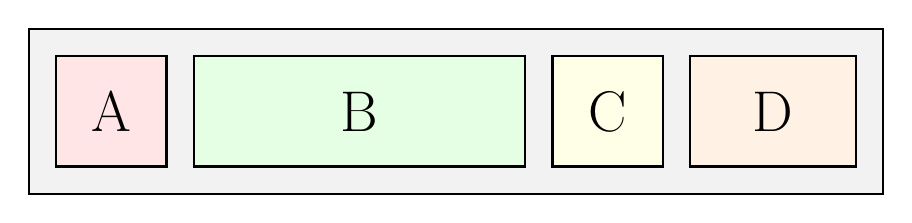
\begin{tikzpicture}[scale=0.07,rotate=0]
		
	%Frame
	\draw[thick, draw=black, fill=gray!10] (0,0) rectangle (155,30);

	%Segments
	%A
	\draw[thick, draw=black, fill=red!10] (5,5) rectangle (25,25);
	\node at (15,15) {\huge A};
	
	%B
	\draw[thick, draw=black, fill=green!10] (30,5) rectangle (90,25);
	\node at (60,15) {\huge B};

	%C
	\draw[thick, draw=black, fill=yellow!10] (95,5) rectangle (115,25);
	\node at (105,15) {\huge C};

	%D
	\draw[thick, draw=black, fill=orange!10] (120,5) rectangle (150,25);
	\node at (135,15) {\huge D};
	
\end{tikzpicture}
\end{document}
